\chapter{Proof for rank 5}

\begin{lemma}
  $\rho_0$ (and thus $\rho_4$) cannot be a 4-transposition.
\end{lemma}

\begin{proof}
  Suppose that $\rho_0$ is a 4-transposition.

  \paragraph{}
  The $\rho_4$ involution must be placed on the graph such that it commutes with $\rho_0$. The following patterns are possible for each $\rho_4$ edge:
  \begin{enumerate}
    \item Form an alternating square
    \item Double an existing edge
    \item Link two fixed points
  \end{enumerate}

  \paragraph{}
  The last pattern can only be used once because there are only three fixed points. But $\rho_4$ is either a 4-transposition or a 2-transposition, so at least one edge that must still be placed. Thus, at least one of the two other possibilities must be used. But $\rho_0$ and $\rho_4$ would share a vertex but that is impossible by Lemma~\ref{0-4-no-share}.
\end{proof}

The analysis is split in two cases depending of the disposition of 4-transpositions:
\begin{enumerate}
  \item $\rho_1$ is a 4-transposition (regardless of $\rho_3$)
  \item $\rho_1$ and $\rho_3$ are 2-transpositions. If $\rho_3$ is a 4-transposition but $\rho_1$ not, it can be reduced to the first case by taking the dual.
\end{enumerate}

\section{$\rho_1$ is a 4-transposition}

\begin{theorem}
  If $\rho_1$ is a 4-transposition, then a generator can be written as a product of other generators, and thus the generating set is not free, and the group is not a sggi.
\end{theorem}

\paragraph{}
Let's draw a graph with all edges of the 4-transposition $\rho_1$.

\begin{figure}[H]
  \begin{center}
    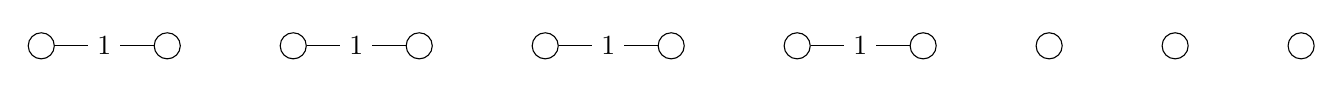
\begin{tikzpicture}[scale=.8]

      \begin{scope}[every node/.style={circle,draw}]
        \node (1)  at (0,0)  {};
        \node (2)  at (2,0)  {};
        \node (3)  at (4,0)  {};
        \node (4)  at (6,0)  {};
        \node (5)  at (8,0)  {};
        \node (6)  at (10,0)  {};
        \node (7)  at (12,0)  {};
        \node (8)  at (14,0)  {};
        \node (9)  at (16,0)  {};
        \node (10) at (18,0)  {};
        \node (11) at (20,0) {};
      \end{scope}

      \begin{scope}[every node/.style={fill=white}]

        \begin{scope}[every edge/.style={draw}]
          \path (1)  edge node {$1$} (2);
          \path (3)  edge node {$1$} (4);
          \path (5)  edge node {$1$} (6);
          \path (7)  edge node {$1$} (8);
        \end{scope}
      \end{scope}

    \end{tikzpicture}
    \caption{}
  \end{center}
\end{figure}

\paragraph{}
This transposition must commute with $\rho_3$ and $\rho_4$. There are three possibilities to place the two $\rho_4$ edges: building an alternating square, doubling one edge a linking two fixed points or doubling two edges.

\subsection{The alternating square}

\begin{figure}[H]
  \begin{center}
    \begin{tikzpicture}[scale=.8]

      \begin{scope}[every node/.style={circle,draw}]
        \node (1)  at (0,2)  {};
        \node (2)  at (0,0)  {};
        \node (3)  at (2,2)  {};
        \node (4)  at (2,0)  {};
        \node (5)  at (4,0)  {};
        \node (6)  at (6,0)  {};
        \node (7)  at (8,0)  {};
        \node (8)  at (10,0)  {};
        \node (9)  at (12,0)  {};
        \node (10) at (14,0)  {};
        \node (11) at (16,0) {};
      \end{scope}

      \begin{scope}[every node/.style={fill=white}]

        \begin{scope}[every edge/.style={draw}]
          \path (1)  edge node {$1$} (2);
          \path (3)  edge node {$1$} (4);
          \path (5)  edge node {$1$} (6);
          \path (7)  edge node {$1$} (8);
          \path (1)  edge node {$4$} (3);
          \path (2)  edge node {$4$} (4);
        \end{scope}
      \end{scope}

    \end{tikzpicture}
    \caption{}
  \end{center}
\end{figure}

\paragraph{}
If $\rho_4$ forms an alternating square with $\rho_1$, it must be adjacent to an other alternating square $[\rho_1, \rho_3]$ ($[\rho_2, \rho_4]$ is not possible because $\rho_4$ is a 2-transposition). The sequence of squares cannot be extended to the right because two extra alternating squares are needed. There is only one remaining $\rho_1$ edge, therefore it is not possible to continue linearly. But a rotation pattern cannot be placed, so it is impossible.

\paragraph{}
If the sequence is extended to the left, the last $\rho_1$ edge and two $\rho_3$ edges would be used. At the end only 2 $\rho_0$ edges and 2 or 4 $\rho_2$ edges remain but they cannot form a connected graph.

\paragraph{}
The sequence of alternating squares must therefore be of length 2. Those squares must be linked to the rest of the graph by a $\rho_2$ edge.

\begin{figure}[H]
  \begin{center}
    \begin{tikzpicture}[scale=.8]

      \begin{scope}[every node/.style={circle,draw}]
        \node (1)  at (0,2)  {};
        \node (2)  at (0,0)  {};
        \node (3)  at (2,2)  {};
        \node (4)  at (2,0)  {};
        \node (5)  at (4,2)  {};
        \node (6)  at (4,0)  {};
        \node (7)  at (6,0)  {};
        \node (8)  at (8,0)  {};
        \node (9)  at (10,0)  {};
        \node (10) at (12,0)  {};
        \node (11) at (14,0) {};
      \end{scope}

      \begin{scope}[every node/.style={fill=white}]

        \begin{scope}[every edge/.style={draw}]
          \path (1)  edge node {$1$} (2);
          \path (3)  edge node {$1$} (4);
          \path (5)  edge node {$1$} (6);
          \path (7)  edge node {$1$} (8);
          \path (3)  edge node {$3$} (5);
          \path (4)  edge node {$3$} (6);
          \path (1)  edge node {$4$} (3);
          \path (2)  edge node {$4$} (4);
        \end{scope}
      \end{scope}

    \end{tikzpicture}
    \caption{}
  \end{center}
\end{figure}


\paragraph{}
By Lemma~\ref{adjacent-must-not-commute} $\rho_0$ and $\rho_1$ must not commute. Thus a $\rho_0$ edge must share a vertex with a $\rho_1$ edge, otherwise $\rho_0$ and $\rho_1$ would commute.

\paragraph{}
By Lemma~\ref{0-4-no-share}, the edges of involutions $\rho_0$ and $\rho_4$ cannot share a vertex. So the $\rho_0$ edge cannot be linked to the first 4 vertices. They cannot be connected thus to the 5th and 6th vertices because it would form an alternating square but it was proved that the sequence cannot be extended.

\paragraph{}
Thus, a $\rho_0$ edge must link the extremity of the single $\rho_1$ edge to a fixed point. The other $\rho_0$ edge must link the two fixed points because if the other extremity of the single $\rho_1$ edge is used, it is not possible to connect the formed component.

\begin{figure}[H]
  \begin{center}
    \begin{tikzpicture}[scale=.8]

      \begin{scope}[every node/.style={circle,draw}]
        \node (1)  at (0,2)  {};
        \node (2)  at (0,0)  {};
        \node (3)  at (2,2)  {};
        \node (4)  at (2,0)  {};
        \node (5)  at (4,2)  {};
        \node (6)  at (4,0)  {};
        \node (7)  at (6,0)  {};
        \node (8)  at (8,0)  {};
        \node (9)  at (10,0)  {};
        \node (10) at (12,0)  {};
        \node (11) at (14,0) {};
      \end{scope}

      \begin{scope}[every node/.style={fill=white}]

        \begin{scope}[every edge/.style={draw}]
          \path (8)  edge node {$0$} (9);
          \path (10)  edge node {$0$} (11);
          \path (1)  edge node {$1$} (2);
          \path (3)  edge node {$1$} (4);
          \path (5)  edge node {$1$} (6);
          \path (7)  edge node {$1$} (8);
          \path (3)  edge node {$3$} (5);
          \path (4)  edge node {$3$} (6);
          \path (1)  edge node {$4$} (3);
          \path (2)  edge node {$4$} (4);
        \end{scope}
      \end{scope}

    \end{tikzpicture}
    \caption{}
  \end{center}
\end{figure}

\paragraph{}
The two alternating squares can only be linked by a $\rho_2$ edge. This edge must be linked to the $\rho_1$ component because it is not possible to continue the sequence.

\begin{figure}[H]
  \begin{center}
    \begin{tikzpicture}[scale=.8]

      \begin{scope}[every node/.style={circle,draw}]
        \node (1)  at (0,2)  {};
        \node (2)  at (0,0)  {};
        \node (3)  at (2,2)  {};
        \node (4)  at (2,0)  {};
        \node (5)  at (4,2)  {};
        \node (6)  at (4,0)  {};
        \node (7)  at (6,0)  {};
        \node (8)  at (8,0)  {};
        \node (9)  at (10,0)  {};
        \node (10) at (12,0)  {};
        \node (11) at (14,0) {};
      \end{scope}

      \begin{scope}[every node/.style={fill=white}]

        \begin{scope}[every edge/.style={draw}]
          \path (8)  edge node {$0$} (9);
          \path (10)  edge node {$0$} (11);
          \path (1)  edge node {$1$} (2);
          \path (3)  edge node {$1$} (4);
          \path (5)  edge node {$1$} (6);
          \path (7)  edge node {$1$} (8);
          \path (6)  edge node {$2$} (7);
          \path (3)  edge node {$3$} (5);
          \path (4)  edge node {$3$} (6);
          \path (1)  edge node {$4$} (3);
          \path (2)  edge node {$4$} (4);
        \end{scope}
      \end{scope}

    \end{tikzpicture}
    \caption{}
  \end{center}
\end{figure}

\paragraph{}
All $\rho_1$ edges have been used, they cannot be used to link the single $\rho_0$. Therefore it is necessary to use an alternating square to connect it. But this alternating square must be connected to a single edge. Therefore the difference between the indices of the edges must be 2. The vertical edges of the square must therefore be $\rho_2$.

\begin{figure}[H]
  \begin{center}
    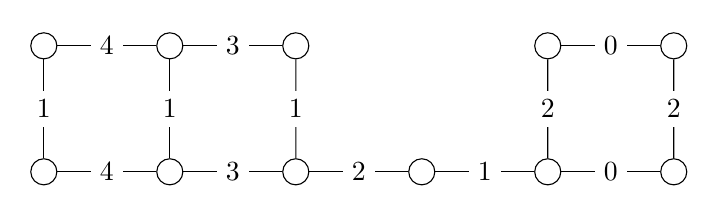
\begin{tikzpicture}[scale=.8]

      \begin{scope}[every node/.style={circle,draw}]
        \node (1)  at (0,2)  {};
        \node (2)  at (0,0)  {};
        \node (3)  at (2,2)  {};
        \node (4)  at (2,0)  {};
        \node (5)  at (4,2)  {};
        \node (6)  at (4,0)  {};
        \node (7)  at (6,0)  {};
        \node (8)  at (8,2)  {};
        \node (9)  at (8,0)  {};
        \node (10) at (10,2)  {};
        \node (11) at (10,0) {};
      \end{scope}

      \begin{scope}[every node/.style={fill=white}]

        \begin{scope}[every edge/.style={draw}]
          \path (9)  edge node {$0$} (11);
          \path (8)  edge node {$0$} (10);
          \path (1)  edge node {$1$} (2);
          \path (3)  edge node {$1$} (4);
          \path (5)  edge node {$1$} (6);
          \path (7)  edge node {$1$} (9);
          \path (6)  edge node {$2$} (7);
          \path (8)  edge node {$2$} (9);
          \path (10) edge node {$2$} (11);
          \path (3)  edge node {$3$} (5);
          \path (4)  edge node {$3$} (6);
          \path (1)  edge node {$4$} (3);
          \path (2)  edge node {$4$} (4);
        \end{scope}
      \end{scope}

    \end{tikzpicture}
    \caption{}
  \end{center}
\end{figure}

\paragraph{}
There are only 3 $\rho_2$ edges on this graph. A last one must be added to restore parity. There are only two places possible: double any of the $\rho_4$ edge. That gives 2 graphs:

\begin{figure}[H]
  \begin{center}
    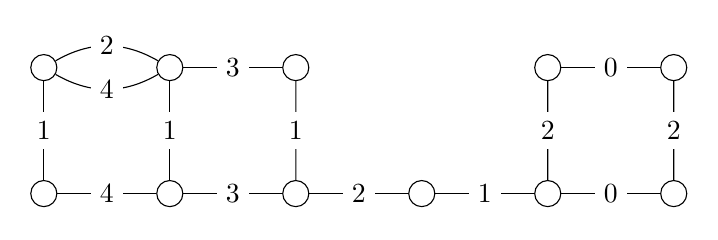
\begin{tikzpicture}[scale=.8]

      \begin{scope}[every node/.style={circle,draw}]
        \node (1)  at (0,2)  {};
        \node (2)  at (0,0)  {};
        \node (3)  at (2,2)  {};
        \node (4)  at (2,0)  {};
        \node (5)  at (4,2)  {};
        \node (6)  at (4,0)  {};
        \node (7)  at (6,0)  {};
        \node (8)  at (8,2)  {};
        \node (9)  at (8,0)  {};
        \node (10) at (10,2)  {};
        \node (11) at (10,0) {};
      \end{scope}

      \begin{scope}[every node/.style={fill=white}]

        \begin{scope}[every edge/.style={draw}]
          \path (9)  edge node {$0$} (11);
          \path (8)  edge node {$0$} (10);
          \path (1)  edge node {$1$} (2);
          \path (3)  edge node {$1$} (4);
          \path (5)  edge node {$1$} (6);
          \path (7)  edge node {$1$} (9);
          \path (1)  edge[bend left=30] node {$2$} (3);
          \path (6)  edge node {$2$} (7);
          \path (8)  edge node {$2$} (9);
          \path (10) edge node {$2$} (11);
          \path (3)  edge node {$3$} (5);
          \path (4)  edge node {$3$} (6);
          \path (1)  edge[bend right=30] node {$4$} (3);
          \path (2)  edge node {$4$} (4);
        \end{scope}
      \end{scope}

    \end{tikzpicture}
    \caption{}
  \end{center}
\end{figure}

\begin{figure}[H]
  \begin{center}
    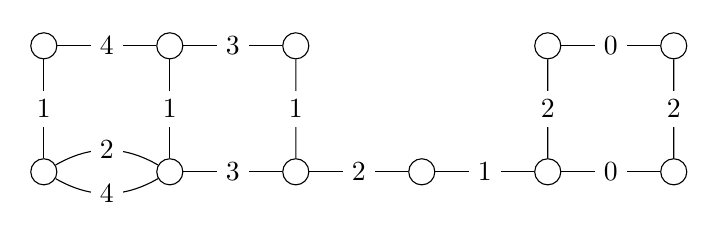
\begin{tikzpicture}[scale=.8]

      \begin{scope}[every node/.style={circle,draw}]
        \node (1)  at (0,2)  {};
        \node (2)  at (0,0)  {};
        \node (3)  at (2,2)  {};
        \node (4)  at (2,0)  {};
        \node (5)  at (4,2)  {};
        \node (6)  at (4,0)  {};
        \node (7)  at (6,0)  {};
        \node (8)  at (8,2)  {};
        \node (9)  at (8,0)  {};
        \node (10) at (10,2)  {};
        \node (11) at (10,0) {};
      \end{scope}

      \begin{scope}[every node/.style={fill=white}]

        \begin{scope}[every edge/.style={draw}]
          \path (9)  edge node {$0$} (11);
          \path (8)  edge node {$0$} (10);
          \path (1)  edge node {$1$} (2);
          \path (3)  edge node {$1$} (4);
          \path (5)  edge node {$1$} (6);
          \path (7)  edge node {$1$} (9);
          \path (2)  edge[bend left=30] node {$2$} (4);
          \path (6)  edge node {$2$} (7);
          \path (8)  edge node {$2$} (9);
          \path (10) edge node {$2$} (11);
          \path (3)  edge node {$3$} (5);
          \path (4)  edge node {$3$} (6);
          \path (1)  edge node {$4$} (3);
          \path (2)  edge[bend right=30] node {$4$} (4);
        \end{scope}
      \end{scope}

    \end{tikzpicture}
    \caption{}
  \end{center}
\end{figure}

\paragraph{}
Those graphs are valid graphs but $\rho_3$ is a 2-transposition. This involution can be extended to a 4-transposition. There are only two possible positions for extra $\rho_3$ edges: double the left $\rho_1$ edge and the upper $\rho_0$ edge. That creates two other graphs:

\begin{figure}[H]
  \begin{center}
    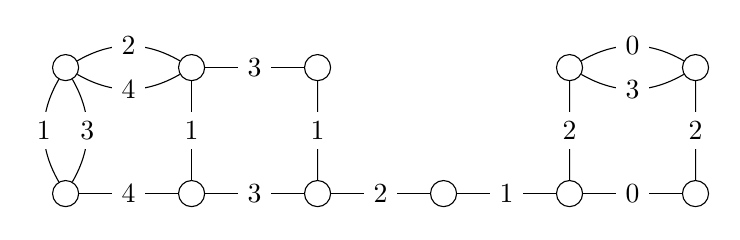
\begin{tikzpicture}[scale=.8]

      \begin{scope}[every node/.style={circle,draw}]
        \node (1)  at (0,2)  {};
        \node (2)  at (0,0)  {};
        \node (3)  at (2,2)  {};
        \node (4)  at (2,0)  {};
        \node (5)  at (4,2)  {};
        \node (6)  at (4,0)  {};
        \node (7)  at (6,0)  {};
        \node (8)  at (8,2)  {};
        \node (9)  at (8,0)  {};
        \node (10) at (10,2)  {};
        \node (11) at (10,0) {};
      \end{scope}

      \begin{scope}[every node/.style={fill=white}]

        \begin{scope}[every edge/.style={draw}]
          \path (9)  edge node {$0$} (11);
          \path (8)  edge[bend left=30] node {$0$} (10);
          \path (1)  edge[bend right=30] node {$1$} (2);
          \path (3)  edge node {$1$} (4);
          \path (5)  edge node {$1$} (6);
          \path (7)  edge node {$1$} (9);
          \path (1)  edge[bend left=30] node {$2$} (3);
          \path (6)  edge node {$2$} (7);
          \path (8)  edge node {$2$} (9);
          \path (10) edge node {$2$} (11);
          \path (1)  edge[bend left=30] node {$3$} (2);
          \path (3)  edge node {$3$} (5);
          \path (4)  edge node {$3$} (6);
          \path (8)  edge[bend right=30] node {$3$} (10);
          \path (1)  edge[bend right=30] node {$4$} (3);
          \path (2)  edge node {$4$} (4);
        \end{scope}
      \end{scope}

    \end{tikzpicture}
    \caption{}
  \end{center}
\end{figure}

\begin{figure}[H]
  \begin{center}
    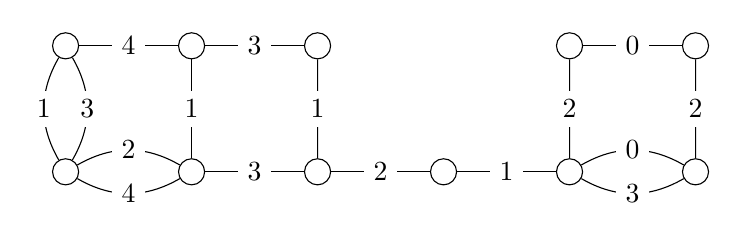
\begin{tikzpicture}[scale=.8]

      \begin{scope}[every node/.style={circle,draw}]
        \node (1)  at (0,2)  {};
        \node (2)  at (0,0)  {};
        \node (3)  at (2,2)  {};
        \node (4)  at (2,0)  {};
        \node (5)  at (4,2)  {};
        \node (6)  at (4,0)  {};
        \node (7)  at (6,0)  {};
        \node (8)  at (8,2)  {};
        \node (9)  at (8,0)  {};
        \node (10) at (10,2)  {};
        \node (11) at (10,0) {};
      \end{scope}

      \begin{scope}[every node/.style={fill=white}]

        \begin{scope}[every edge/.style={draw}]
          \path (9)  edge[bend left=30] node {$0$} (11);
          \path (8)  edge node {$0$} (10);
          \path (1)  edge[bend right=30] node {$1$} (2);
          \path (3)  edge node {$1$} (4);
          \path (5)  edge node {$1$} (6);
          \path (7)  edge node {$1$} (9);
          \path (2)  edge[bend left=30] node {$2$} (4);
          \path (6)  edge node {$2$} (7);
          \path (8)  edge node {$2$} (9);
          \path (10) edge node {$2$} (11);
          \path (1)  edge[bend left=30] node {$3$} (2);
          \path (3)  edge node {$3$} (5);
          \path (4)  edge node {$3$} (6);
          \path (9)  edge[bend right=30] node {$3$} (11);
          \path (1)  edge node {$4$} (3);
          \path (2)  edge[bend right=30] node {$4$} (4);
        \end{scope}
      \end{scope}

    \end{tikzpicture}
    \caption{}
  \end{center}
\end{figure}

\paragraph{}
Let's remove all edges from involutions $\rho_0$ and $\rho_3$:

\begin{figure}[H]
  \begin{center}
    \begin{tikzpicture}[scale=.8]

      \begin{scope}[every node/.style={circle,draw}]
        \node (1)  at (0,2)  {};
        \node (2)  at (0,0)  {};
        \node (3)  at (2,2)  {};
        \node (4)  at (2,0)  {};
        \node (5)  at (6,0)  {};
        \node (6)  at (4,0)  {};
        \node (7)  at (8,0)  {};
        \node (8)  at (10,0)  {};
        \node (9)  at (12,0)  {};
        \node (10) at (14,0)  {};
        \node (11) at (16,0) {};
      \end{scope}

      \begin{scope}[every node/.style={fill=white}]

        \begin{scope}[every edge/.style={draw}]
          \path (1)  edge node {$1$} (2);
          \path (3)  edge node {$1$} (4);
          \path (5)  edge node {$1$} (6);
          \path (7)  edge node {$1$} (8);
          \path (1)  edge[bend left=30] node {$2$} (3);
          \path (5)  edge node {$2$} (7);
          \path (8)  edge node {$2$} (9);
          \path (10) edge node {$2$} (11);
          \path (1)  edge[bend right=30] node {$4$} (3);
          \path (2)  edge node {$4$} (4);
        \end{scope}
      \end{scope}

    \end{tikzpicture}
    \caption{}
  \end{center}
\end{figure}

\paragraph{}
Now it can easily be seen that $\rho_4 = (\rho_1 \rho_2)^{10}$. Thus none of those four graphs have a free set of generators and so none of then are sggis.

\section{A double edge and a single edge between two fixed points}

\paragraph{}
The second possibility is having a double edge $(\rho_0, \rho_4)$. By Lemma~\ref{todo}, an alternating square must be placed next to it in order to allow it to be connected to the rest of the graph. There are possibilities for the alternating square: $[\rho_1, \rho_3]$ or $[\rho_2, \rho_4]$.
\subsection{Alternating square $[\rho_1, \rho_3]$}

\begin{figure}[H]
  \begin{center}
    \begin{tikzpicture}[scale=.8]

      \begin{scope}[every node/.style={circle,draw}]
        \node (1)  at (0,2)  {};
        \node (2)  at (0,0)  {};
        \node (3)  at (2,2)  {};
        \node (4)  at (2,0)  {};
        \node (5)  at (4,0)  {};
        \node (6)  at (6,0)  {};
        \node (7)  at (8,0)  {};
        \node (8)  at (10,0)  {};
        \node (9)  at (12,0)  {};
        \node (10) at (14,0)  {};
        \node (11) at (16,0) {};
      \end{scope}

      \begin{scope}[every node/.style={fill=white}]

        \begin{scope}[every edge/.style={draw}]
          \path (1)  edge[bend right=30] node {$1$} (2);
          \path (3)  edge node {$1$} (4);
          \path (5)  edge node {$1$} (6);
          \path (7)  edge node {$1$} (8);
          \path (1)  edge node {$3$} (3);
          \path (2)  edge node {$3$} (4);
          \path (1)  edge[bend left=30] node {$4$} (2);
        \end{scope}
      \end{scope}

    \end{tikzpicture}
    \caption{}
  \end{center}
\end{figure}

\paragraph{}
By lemma~\ref{todo}, $\rho_0$ and $\rho_1$ must not commute. A $\rho_0$ edge must thus be connected to at least one $\rho_1$ edge. So at least one $\rho_1$ edge must not be part of an alternating square of which $\rho_0$ does not belong.

\paragraph{}
This alternating square cannot be linked by another alternating square on the right because it will need two alternating squares on the right if the value of the vertical edges is not changed. But that uses all $\rho_1$ in alternating squares, which is not possible by the previous statement.

\paragraph{}
The values of the vertical edges must therefore be changed. The horizontal edges of the second square must be $\rho_2$ because the involutions must be adjacent to $\rho_3$ and there is not enough $\rho_4$ edges. Then the new value for vertical edge must be adjacent to $\rho_3$. $\rho_2$ is impossible because it is already used for the horizontal edges. The only remaining possibility is $\rho_4$ but there are no enough remaining edges.

\paragraph{}
If an alternating square is attached on the left, it must be $[\rho_2, \rho_4]$.

\begin{figure}[H]
  \begin{center}
    \begin{tikzpicture}[scale=.8]

      \begin{scope}[every node/.style={circle,draw}]
        \node (1)  at (0,2)  {};
        \node (2)  at (0,0)  {};
        \node (3)  at (2,2)  {};
        \node (4)  at (2,0)  {};
        \node (5)  at (4,0)  {};
        \node (6)  at (6,0)  {};
        \node (7)  at (8,0)  {};
        \node (8)  at (10,0)  {};
        \node (9)  at (-2,2)  {};
        \node (10) at (-2,0)  {};
        \node (11) at (12,0) {};
      \end{scope}

      \begin{scope}[every node/.style={fill=white}]

        \begin{scope}[every edge/.style={draw}]
          \path (1)  edge[bend right=30] node {$1$} (2);
          \path (3)  edge node {$1$} (4);
          \path (5)  edge node {$1$} (6);
          \path (7)  edge node {$1$} (8);
          \path (1)  edge node {$2$} (9);
          \path (2)  edge node {$2$} (10);
          \path (1)  edge node {$3$} (3);
          \path (2)  edge node {$3$} (4);
          \path (1)  edge[bend left=30] node {$4$} (2);
          \path (9)  edge node {$4$} (10);
        \end{scope}
      \end{scope}

    \end{tikzpicture}
    \caption{}
  \end{center}
\end{figure}

\paragraph{}
The two $\rho_0$ edges cannot be placed on any vertex of the left component. If the fixed point is not used to connect the $\rho_0$ edges, the two $\rho_1$ edges must be linked together twice and thus build an alternating square. Then $\rho_0$ and $\rho_1$ commute and that is impossible. Thus the fixed point must be connected by $\rho_0$.

\paragraph{}
The first $\rho_0$ edge must connect the fixed point to a $\rho_1$ edge and the second must connect the two $\rho_1$ edges together.

\begin{figure}[H]
  \begin{center}
    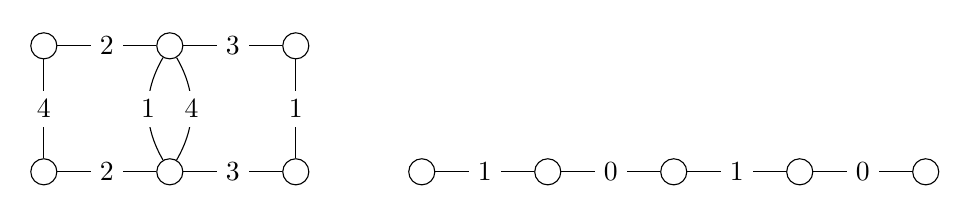
\begin{tikzpicture}[scale=.8]

      \begin{scope}[every node/.style={circle,draw}]
        \node (1)  at (0,2)  {};
        \node (2)  at (0,0)  {};
        \node (3)  at (2,2)  {};
        \node (4)  at (2,0)  {};
        \node (5)  at (4,0)  {};
        \node (6)  at (6,0)  {};
        \node (7)  at (8,0)  {};
        \node (8)  at (10,0)  {};
        \node (9)  at (-2,2)  {};
        \node (10) at (-2,0)  {};
        \node (11) at (12,0) {};
      \end{scope}

      \begin{scope}[every node/.style={fill=white}]

        \begin{scope}[every edge/.style={draw}]
          \path (6)  edge node {$0$} (7);
          \path (8)  edge node {$0$} (11);
          \path (1)  edge[bend right=30] node {$1$} (2);
          \path (3)  edge node {$1$} (4);
          \path (5)  edge node {$1$} (6);
          \path (7)  edge node {$1$} (8);
          \path (1)  edge node {$2$} (9);
          \path (2)  edge node {$2$} (10);
          \path (1)  edge node {$3$} (3);
          \path (2)  edge node {$3$} (4);
          \path (1)  edge[bend left=30] node {$4$} (2);
          \path (9)  edge node {$4$} (10);
        \end{scope}
      \end{scope}

    \end{tikzpicture}
    \caption{}
  \end{center}
\end{figure}

\paragraph{}
Two components must be linked by a $\rho_2$ edge. But the total number of $\rho_2$ edges becomes odd. Another $\rho_2$ must thus be placed. The only possibilities are to double a $\rho_0$ edge. There are two possible graphs:

\begin{figure}[H]
  \begin{center}
    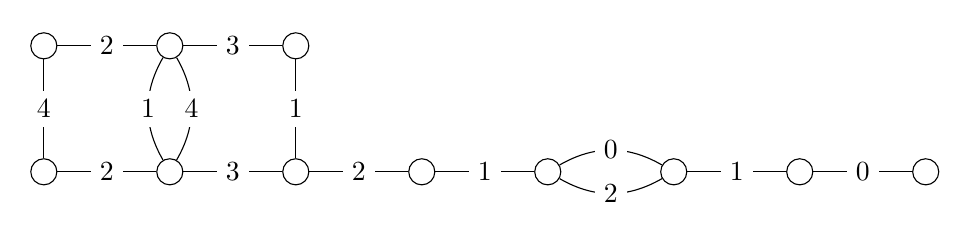
\begin{tikzpicture}[scale=.8]

      \begin{scope}[every node/.style={circle,draw}]
        \node (1)  at (0,2)  {};
        \node (2)  at (0,0)  {};
        \node (3)  at (2,2)  {};
        \node (4)  at (2,0)  {};
        \node (5)  at (4,0)  {};
        \node (6)  at (6,0)  {};
        \node (7)  at (8,0)  {};
        \node (8)  at (10,0)  {};
        \node (9)  at (-2,2)  {};
        \node (10) at (-2,0)  {};
        \node (11) at (12,0) {};
      \end{scope}

      \begin{scope}[every node/.style={fill=white}]

        \begin{scope}[every edge/.style={draw}]
          \path (6)  edge[bend left=30] node {$0$} (7);
          \path (8)  edge node {$0$} (11);
          \path (1)  edge[bend right=30] node {$1$} (2);
          \path (3)  edge node {$1$} (4);
          \path (5)  edge node {$1$} (6);
          \path (7)  edge node {$1$} (8);
          \path (1)  edge node {$2$} (9);
          \path (2)  edge node {$2$} (10);
          \path (4)  edge node {$2$} (5);
          \path (6)  edge[bend right=30] node {$2$} (7);
          \path (1)  edge node {$3$} (3);
          \path (2)  edge node {$3$} (4);
          \path (1)  edge[bend left=30] node {$4$} (2);
          \path (9)  edge node {$4$} (10);
        \end{scope}
      \end{scope}

    \end{tikzpicture}
    \caption{}
  \end{center}
\end{figure}

\begin{figure}[H]
  \begin{center}
    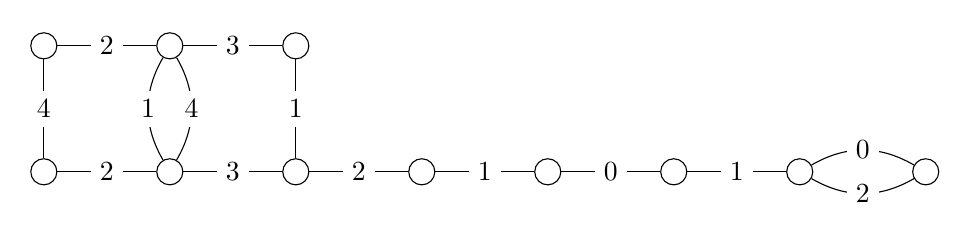
\begin{tikzpicture}[scale=.8]

      \begin{scope}[every node/.style={circle,draw}]
        \node (1)  at (0,2)  {};
        \node (2)  at (0,0)  {};
        \node (3)  at (2,2)  {};
        \node (4)  at (2,0)  {};
        \node (5)  at (4,0)  {};
        \node (6)  at (6,0)  {};
        \node (7)  at (8,0)  {};
        \node (8)  at (10,0)  {};
        \node (9)  at (-2,2)  {};
        \node (10) at (-2,0)  {};
        \node (11) at (12,0) {};
      \end{scope}

      \begin{scope}[every node/.style={fill=white}]

        \begin{scope}[every edge/.style={draw}]
          \path (6)  edge node {$0$} (7);
          \path (8)  edge[bend left=30] node {$0$} (11);
          \path (1)  edge[bend right=30] node {$1$} (2);
          \path (3)  edge node {$1$} (4);
          \path (5)  edge node {$1$} (6);
          \path (7)  edge node {$1$} (8);
          \path (1)  edge node {$2$} (9);
          \path (2)  edge node {$2$} (10);
          \path (4)  edge node {$2$} (5);
          \path (8)  edge[bend right=30] node {$2$} (11);
          \path (1)  edge node {$3$} (3);
          \path (2)  edge node {$3$} (4);
          \path (1)  edge[bend left=30] node {$4$} (2);
          \path (9)  edge node {$4$} (10);
        \end{scope}
      \end{scope}

    \end{tikzpicture}
    \caption{}
  \end{center}
\end{figure}

\paragraph{}
In those graphs, if the $\rho_4$ edge is removed, the generated group is 2-transitive\footnote{TO DO} and thus primitive. By looking at the size of the subgroups, it is possible to deduce that the generated group is $A_{11}$\footnote{Missing the case where no other square are attached}.

\subsection{Alternating square $[\rho_2,\rho_4]$}

\begin{figure}[H]
  \begin{center}
    \begin{tikzpicture}[scale=.8]

      \begin{scope}[every node/.style={circle,draw}]
        \node (1)  at (0,2)  {};
        \node (2)  at (0,0)  {};
        \node (3)  at (2,2)  {};
        \node (4)  at (2,0)  {};
        \node (5)  at (6,0)  {};
        \node (6)  at (4,0)  {};
        \node (7)  at (10,0)  {};
        \node (8)  at (8,0)  {};
        \node (9)  at (12,0)  {};
        \node (10) at (14,0)  {};
        \node (11) at (16,0) {};
      \end{scope}

      \begin{scope}[every node/.style={fill=white}]

        \begin{scope}[every edge/.style={draw}]
          \path (1)  edge[bend right=30] node {$1$} (2);
          \path (5)  edge node {$1$} (6);
          \path (7)  edge node {$1$} (8);
          \path (9)  edge node {$1$} (10);
          \path (1)  edge node {$2$} (3);
          \path (2)  edge node {$2$} (4);
          \path (1)  edge[bend left=30] node {$4$} (2);
          \path (3)  edge node {$4$} (4);
        \end{scope}
      \end{scope}

    \end{tikzpicture}
    \caption{}
  \end{center}
\end{figure}

\paragraph{}
Either two extra alternating squares can be added or this alternating square can be linked to some other component.

\paragraph{}
In the first case, it is impossible to add another alternating square to right of this sequence.

\paragraph{}
The alternating square can however be extended to the left by a $[\rho_1, \rho_3]$ edge but then it can be reduced to the $[\rho_1, \rho_3]$ case.

\paragraph{}
The only remaining possibility is to link to square to the rest of the graph with a single edge. A $\rho_3$ edge must be used. It cannot be connected to a $\rho_1$ edge an alternating square should be built but that is impossible. The only possibility is to link it to the fixed point.

\begin{figure}[H]
  \begin{center}
    \begin{tikzpicture}[scale=.8]

      \begin{scope}[every node/.style={circle,draw}]
        \node (1)  at (0,2)  {};
        \node (2)  at (0,0)  {};
        \node (3)  at (2,2)  {};
        \node (4)  at (2,0)  {};
        \node (5)  at (8,0)  {};
        \node (6)  at (6,0)  {};
        \node (7)  at (12,0)  {};
        \node (8)  at (10,0)  {};
        \node (9)  at (14,0)  {};
        \node (10) at (16,0)  {};
        \node (11) at (4,0) {};
      \end{scope}

      \begin{scope}[every node/.style={fill=white}]

        \begin{scope}[every edge/.style={draw}]
          \path (1)  edge[bend right=30] node {$1$} (2);
          \path (5)  edge node {$1$} (6);
          \path (7)  edge node {$1$} (8);
          \path (9)  edge node {$1$} (10);
          \path (1)  edge node {$2$} (3);
          \path (2)  edge node {$2$} (4);
          \path (4)  edge node {$3$} (11);
          \path (1)  edge[bend left=30] node {$4$} (2);
          \path (3)  edge node {$4$} (4);
        \end{scope}
      \end{scope}

    \end{tikzpicture}
    \caption{}
  \end{center}
\end{figure}

\paragraph{}
Two $\rho_0$ edges must still be placed and they must not commute with $\rho_1$. Thus at least one edge must link two $\rho_1$ involutions. And the other $\rho_0$ edge must link the two other $\rho_1$ edges.

\begin{figure}[H]
  \begin{center}
    \begin{tikzpicture}[scale=.8]

      \begin{scope}[every node/.style={circle,draw}]
        \node (1)  at (0,2)  {};
        \node (2)  at (0,0)  {};
        \node (3)  at (2,2)  {};
        \node (4)  at (2,0)  {};
        \node (5)  at (8,0)  {};
        \node (6)  at (6,0)  {};
        \node (7)  at (12,0)  {};
        \node (8)  at (10,0)  {};
        \node (9)  at (14,0)  {};
        \node (10) at (16,0)  {};
        \node (11) at (4,0) {};
      \end{scope}

      \begin{scope}[every node/.style={fill=white}]

        \begin{scope}[every edge/.style={draw}]
          \path (5)  edge node {$0$} (8);
          \path (7)  edge node {$0$} (9);
          \path (1)  edge[bend right=30] node {$1$} (2);
          \path (5)  edge node {$1$} (6);
          \path (7)  edge node {$1$} (8);
          \path (9)  edge node {$1$} (10);
          \path (1)  edge node {$2$} (3);
          \path (2)  edge node {$2$} (4);
          \path (4)  edge node {$3$} (11);
          \path (1)  edge[bend left=30] node {$4$} (2);
          \path (3)  edge node {$4$} (4);
        \end{scope}
      \end{scope}

    \end{tikzpicture}
    \caption{}
  \end{center}
\end{figure}

\paragraph{}
Since all $\rho_4$ edge have been used and since no $\rho_2$ can be connected to the alternating square, a $\rho_2$ edge must be used to connect the two components together.

\begin{figure}[H]
  \begin{center}
    \begin{tikzpicture}[scale=.8]

      \begin{scope}[every node/.style={circle,draw}]
        \node (1)  at (0,2)  {};
        \node (2)  at (0,0)  {};
        \node (3)  at (2,2)  {};
        \node (4)  at (2,0)  {};
        \node (5)  at (8,0)  {};
        \node (6)  at (6,0)  {};
        \node (7)  at (12,0)  {};
        \node (8)  at (10,0)  {};
        \node (9)  at (14,0)  {};
        \node (10) at (16,0)  {};
        \node (11) at (4,0) {};
      \end{scope}

      \begin{scope}[every node/.style={fill=white}]

        \begin{scope}[every edge/.style={draw}]
          \path (5)  edge node {$0$} (8);
          \path (7)  edge node {$0$} (9);
          \path (1)  edge[bend right=30] node {$1$} (2);
          \path (5)  edge node {$1$} (6);
          \path (7)  edge node {$1$} (8);
          \path (9)  edge node {$1$} (10);
          \path (1)  edge node {$2$} (3);
          \path (2)  edge node {$2$} (4);
          \path (11)  edge node {$2$} (6);
          \path (4)  edge node {$3$} (11);
          \path (1)  edge[bend left=30] node {$4$} (2);
          \path (3)  edge node {$4$} (4);
        \end{scope}
      \end{scope}

    \end{tikzpicture}
    \caption{}
  \end{center}
\end{figure}

\paragraph{}
The $\rho_3$ involution is currently odd. An extra $\rho_3$ edge must be placed. The only possibility is to triple the double edge. The missing $\rho_2$ edge must then be placed such that a $\rho_0$ edge is doubled. There are two graphs:


\begin{figure}[H]
  \begin{center}
    \begin{tikzpicture}[scale=.8]

      \begin{scope}[every node/.style={circle,draw}]
        \node (1)  at (0,2)  {};
        \node (2)  at (0,0)  {};
        \node (3)  at (2,2)  {};
        \node (4)  at (2,0)  {};
        \node (5)  at (8,0)  {};
        \node (6)  at (6,0)  {};
        \node (7)  at (12,0)  {};
        \node (8)  at (10,0)  {};
        \node (9)  at (14,0)  {};
        \node (10) at (16,0)  {};
        \node (11) at (4,0) {};
      \end{scope}

      \begin{scope}[every node/.style={fill=white}]

        \begin{scope}[every edge/.style={draw}]
          \path (5)  edge[bend left=30] node {$0$} (8);
          \path (7)  edge node {$0$} (9);
          \path (1)  edge[bend right=40] node {$1$} (2);
          \path (5)  edge node {$1$} (6);
          \path (7)  edge node {$1$} (8);
          \path (9)  edge node {$1$} (10);
          \path (1)  edge node {$2$} (3);
          \path (2)  edge node {$2$} (4);
          \path (5)  edge[bend right=30] node {$2$} (8);
          \path (11) edge node {$2$} (6);
          \path (1)  edge node {$3$} (2);
          \path (4)  edge node {$3$} (11);
          \path (1)  edge[bend left=40] node {$4$} (2);
          \path (3)  edge node {$4$} (4);
        \end{scope}
      \end{scope}

    \end{tikzpicture}
    \caption{}
  \end{center}
\end{figure}

\begin{figure}[H]
  \begin{center}
    \begin{tikzpicture}[scale=.8]

      \begin{scope}[every node/.style={circle,draw}]
        \node (1)  at (0,2)  {};
        \node (2)  at (0,0)  {};
        \node (3)  at (2,2)  {};
        \node (4)  at (2,0)  {};
        \node (5)  at (8,0)  {};
        \node (6)  at (6,0)  {};
        \node (7)  at (12,0)  {};
        \node (8)  at (10,0)  {};
        \node (9)  at (14,0)  {};
        \node (10) at (16,0)  {};
        \node (11) at (4,0) {};
      \end{scope}

      \begin{scope}[every node/.style={fill=white}]

        \begin{scope}[every edge/.style={draw}]
          \path (5)  edge node {$0$} (8);
          \path (7)  edge[bend left=30] node {$0$} (9);
          \path (1)  edge[bend right=40] node {$1$} (2);
          \path (5)  edge node {$1$} (6);
          \path (7)  edge node {$1$} (8);
          \path (9)  edge node {$1$} (10);
          \path (1)  edge node {$2$} (3);
          \path (2)  edge node {$2$} (4);
          \path (7)  edge[bend right=30] node {$2$} (9);
          \path (11) edge node {$2$} (6);
          \path (1)  edge node {$3$} (2);
          \path (4)  edge node {$3$} (11);
          \path (1)  edge[bend left=40] node {$4$} (2);
          \path (3)  edge node {$4$} (4);
        \end{scope}
      \end{scope}

    \end{tikzpicture}
    \caption{}
  \end{center}
\end{figure}

\paragraph{}
There are no possibility to convert $\rho_3$ to a 4-transposition in this case.

\paragraph{}
The $\rho_0$ and $\rho_3$ edges can be removed and the obtained graph is the same as those obtained for the alternating square $[\rho_1,\rho_4]$. The consequence are the same: $\rho_4 = (\rho_1\rho_2)^{10}$. The group represented by the previous graphs are therefore not sggi.

\section{Two double edges}

\paragraph{}
The double edges must be contained into alternating squares.

\paragraph{}
If the double edges are placed on the same alternating square, it has already been proved that this does not lead anywhere\footnote{This proof has been deleted}.

\paragraph{}
If the two double edges are place on two different squares, those squares use eight points out of eleven. But it is not possible to place the $\rho_0$ edges such that they do not touch any alternating square.

\section{$\rho_1$ is not a 4-transposition}

\paragraph{}
By Lemma~\ref{min-4-trans}, at least one 4-transposition is needed. It cannot be at the $\rho_1$ position ($\rho_3$ is impossible too by duality). Therefore, $\rho_2$ must be the 4-transposition.

\paragraph{}
In this case, no generator can be omitted. Thus, if one generator is removed, the remaining group would be a sggi of rank 4 with a single 4-transposition but Lemma~\ref{min-4-trans} proved that it cannot generate $A_{11}$.

\begin{theorem}
  The only permutation representation graph of rank 5 on 11 points are those displayed in appendix~\ref{monodromy-5} (p.~\pageref{monodromy-5}).
\end{theorem}

\begin{proof}
  All the possibilities for the permutation representation graphs will be built. The graph with only the 4-transposition $\rho_2$ looks like this:

  \begin{figure}[H]
    \begin{center}
      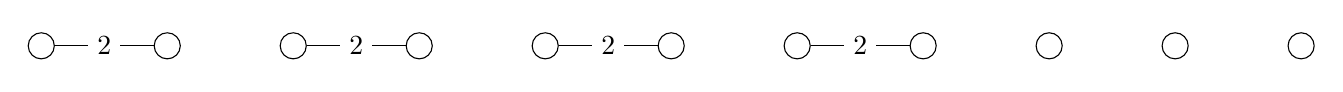
\begin{tikzpicture}[scale=.8]

        \begin{scope}[every node/.style={circle,draw}]
          \node (1)  at (-2,0)  {};
          \node (2)  at (0,0)  {};
          \node (3)  at (2,0)  {};
          \node (4)  at (4,0)  {};
          \node (5)  at (6,0)  {};
          \node (6)  at (8,0)  {};
          \node (7)  at (10,0)  {};
          \node (8)  at (12,0)  {};
          \node (9)  at (14,0)  {};
          \node (10)  at (16,0)  {};
          \node (11)  at (18,0)  {};
        \end{scope}

        \begin{scope}[every node/.style={fill=white}]

          \begin{scope}[every edge/.style={draw}]
            \path (1)  edge node {$2$} (2);
            \path (3)  edge node {$2$} (4);
            \path (5)  edge node {$2$} (6);
            \path (7)  edge node {$2$} (8);
          \end{scope}
        \end{scope}

      \end{tikzpicture}
      \caption{[1, 5, 1010, 232, 381]}
    \end{center}
  \end{figure}

\paragraph{}
If the involutions $\rho_0$ and $\rho_4$ are added to the graph, they must commute with $\rho_2$ and so the only possibilities are:
\begin{enumerate}
  \item A double edge with $\rho_2$ and link two currently fixed points.
  \item Two double edges with $\rho_2$.
  \item An alternating square with $\rho_2$.
\end{enumerate}

\paragraph{}
Since there is only one 4-transposition, there are only 12 edges to link 11 points, 2 more than the minimum. Thus if a edge is added, it must link two distinct components, expect two times. Those two edges are called "joker" edges. When an alternating square is built, one of those edge is used, it is the same if a double edge is built.

\paragraph{}
Among the three possibilities, the second is impossible because, if it is used, even once, it uses both "joker" edges and it is not possible to place the other involution.

\paragraph{}
The same choice cannot be made for $\rho_0$ and $\rho_4$. The first proposition cannot be used twice because it links two fixed points. There are only three of them and so it cannot be used two times.

\paragraph{}
If the third proposition is used twice, there are two alternating squares. If those squares does not share a vertex, they cannot be linked. Thus one square must be linked to the rest of the graph by a $\rho_1$ edge and the other by a $\rho_3$. But those two edges cannot be linked because all $\rho_2$ have already be used and no more alternating square or double edges cannot be used.

\paragraph{}
If the two squares share an edge, a $\rho_0$ and a $\rho_4$ edge are next to each other but that is impossible by Lemma~\ref{0-4-no-share}.

\paragraph{}
The two squares cannot share all their vertices because it will not be able to be connected two the rest of the graph.

\paragraph{}
Thus one of the involution must build an alternating square and the other must build a double edge and links two fixed points. By duality, only the case where $\rho_4$ makes an alternating square will be considered and the other doubles an edge and links two fixed points.

\begin{figure}[H]
  \begin{center}
    \begin{tikzpicture}[scale=.8]

      \begin{scope}[every node/.style={circle,draw}]
        \node (1)  at (12,2)  {};
        \node (2)  at (12,0)  {};
        \node (3)  at (14,2)  {};
        \node (4)  at (14,0)  {};
        \node (5)  at (6,0)  {};
        \node (6)  at (4,0)  {};
        \node (7)  at (10,0)  {};
        \node (8)  at (8,0)  {};
        \node (9)  at (2,0)  {};
        \node (10) at (0,0)  {};
        \node (11) at (16,0) {};
      \end{scope}

      \begin{scope}[every node/.style={fill=white}]

        \begin{scope}[every edge/.style={draw}]
          \path (9)  edge node {$0$} (10);
          \path (7)  edge[bend right=30] node {$0$} (8);
          \path (1)  edge node {$2$} (2);
          \path (3)  edge node {$2$} (4);
          \path (5)  edge node {$2$} (6);
          \path (7)  edge[bend left=30] node {$2$} (8);
          \path (1)  edge node {$4$} (3);
          \path (2)  edge node {$4$} (4);
        \end{scope}
      \end{scope}

    \end{tikzpicture}
    \caption{The graph with only $\rho_0$ and $\rho_2$}
  \end{center}
\end{figure}

\paragraph{}
Now that all of our "joker" edges has been used, every other edge must link two different connected components of the graph.

\paragraph{}
Now the $\rho_3$ edge will be placed. It cannot be adjacent to the component consisting of the single $\rho_0$ edge or to the double edge. There are only three components that can be adjacent to such edge. Thus there are three places for two edges. The component that we are currently building must be linked to the rest of the graph by $\rho_1$ edges and a $\rho_1$ edge can only be connected to the single $\rho_2$ edge. This edge must so be connected by only one $\rho_3$ edge. The same applies for the fixed point that cannot be connected two times, otherwise two $\rho_3$ edges will share this vertex.

\paragraph{}
The square must thus be connected twice. There are three possibilities: the two connected vertices can be opposed or adjacent and, in this case, separated by a $\rho_1$ or a $\rho_3$ edge. This does not influence the position of the $\rho_1$ edges. It is possible to continue building the graph without having to deal with cases. Here is one of the possible graphs:

\begin{figure}[H]
  \begin{center}
    \begin{tikzpicture}[scale=.8]

      \begin{scope}[every node/.style={circle,draw}]
        \node (1)  at (0,2)  {};
        \node (2)  at (0,0)  {};
        \node (3)  at (-2,2)  {};
        \node (4)  at (-2,0)  {};
        \node (5)  at (-6,0)  {};
        \node (6)  at (-4,0)  {};
        \node (7)  at (-10,0)  {};
        \node (8)  at (-8,0)  {};
        \node (9)  at (-14,0)  {};
        \node (10) at (-12,0)  {};
        \node (11) at (2,0) {};
      \end{scope}

      \begin{scope}[every node/.style={fill=white}]

        \begin{scope}[every edge/.style={draw}]
          \path (9)  edge node {$0$} (10);
          \path (7)  edge[bend right=30] node {$0$} (8);
          \path (1)  edge node {$2$} (2);
          \path (3)  edge node {$2$} (4);
          \path (5)  edge node {$2$} (6);
          \path (7)  edge[bend left=30] node {$2$} (8);
          \path (2)  edge node {$3$} (11);
          \path (4)  edge node {$3$} (6);
          \path (1)  edge node {$4$} (3);
          \path (2)  edge node {$4$} (4);
        \end{scope}
      \end{scope}

    \end{tikzpicture}
    \caption{One of the graphs after placing $\rho_3$ edges}
  \end{center}
\end{figure}

\paragraph{}
Now the two edges of $\rho_1$ must be placed, the component containing the alternating square must be attached by its left end, the one that ends with a $\rho_2$ edge. The first two components must be linked together. The first component can be attached in two ways depending on the end choose to be attached. Here is one of the graphs:

\begin{figure}[H]
  \begin{center}
    \begin{tikzpicture}[scale=.8]

      \begin{scope}[every node/.style={circle,draw}]
        \node (1)  at (0,2)  {};
        \node (2)  at (0,0)  {};
        \node (3)  at (-2,2)  {};
        \node (4)  at (-2,0)  {};
        \node (5)  at (-6,0)  {};
        \node (6)  at (-4,0)  {};
        \node (7)  at (-10,0)  {};
        \node (8)  at (-8,0)  {};
        \node (9)  at (-14,0)  {};
        \node (10) at (-12,0)  {};
        \node (11) at (2,0) {};
      \end{scope}

      \begin{scope}[every node/.style={fill=white}]

        \begin{scope}[every edge/.style={draw}]
          \path (9)  edge node {$0$} (10);
          \path (7)  edge[bend left=30] node {$0$} (8);
          \path (5)  edge node {$1$} (8);
          \path (7)  edge node {$1$} (10);
          \path (1)  edge node {$2$} (2);
          \path (3)  edge node {$2$} (4);
          \path (5)  edge node {$2$} (6);
          \path (7)  edge[bend right=30] node {$2$} (8);
          \path (2)  edge node {$3$} (11);
          \path (4)  edge node {$3$} (6);
          \path (1)  edge node {$4$} (3);
          \path (2)  edge node {$4$} (4);
        \end{scope}
      \end{scope}

    \end{tikzpicture}
    \caption{One sggi on $A_{11}$ of rank 5}
  \end{center}
\end{figure}

\paragraph{}
There are 6 possible graphs but only one was built. The construction of the five remaining graphs is left to the reader. He can check that the graphs built match the graphs of appendix~\ref{monodromy-5}.

\end{proof}


\begin{theorem}
  None of the groups represented by the graphs of appendix~\ref{monodromy-5} are C-groups.
\end{theorem}

\begin{proof}
  By the definition of a C-group, it is sufficient to find two subsets of generators $S_1$ and $S_2$ such that $\Gamma_{S_1} \cap \Gamma_{S_2} \neq \Gamma_{S_1 \cap S_2}$.

  \paragraph{}
  This proof is inspired by the section 4 of~\cite{leemansTransactions}.

  \paragraph{}
  In this case, they will be choose $S_1 = \{\rho_1, \rho_2\}$ and $S_2 = \{\rho_2, \rho_3, \rho_4\}$. Here $S_1 \cap S_2 = \{\rho_2\}$ and so $\Gamma_{S_1 \cap S_2} = \Gamma_{\rho_2}$ is a cyclic group of order 2. Hence, $\rho_2$ is an involution.

  \paragraph{}
  $S_1$ will be studied more deeply, only the $\rho_1$ and $\rho_2$ edges are kept in all the possible graphs. There are only two possible graphs:

  \begin{figure}[H]
    \begin{center}
      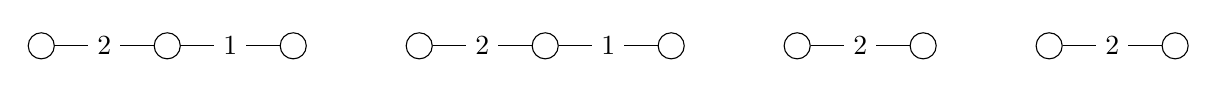
\begin{tikzpicture}[scale=.8]

        \begin{scope}[every node/.style={circle,draw}]
          \node (1)  at (-2,0)  {};
          \node (2)  at (0,0)  {};
          \node (3)  at (2,0)  {};
          \node (4)  at (8,0)  {};
          \node (5)  at (6,0)  {};
          \node (6)  at (4,0)  {};
          \node (7)  at (12,0)  {};
          \node (8)  at (10,0)  {};
          \node (9)  at (16,0)  {};
          \node (10) at (14,0)  {};
        \end{scope}

        \begin{scope}[every node/.style={fill=white}]

          \begin{scope}[every edge/.style={draw}]
            \path (2)  edge node {$1$} (3);
            \path (4)  edge node {$1$} (5);
            \path (1)  edge node {$2$} (2);
            \path (5)  edge node {$2$} (6);
            \path (7)  edge node {$2$} (8);
            \path (9)  edge node {$2$} (10);
          \end{scope}
        \end{scope}

      \end{tikzpicture}
      \caption{First possibility for $\Gamma_{S_1}$}
    \end{center}
  \end{figure}

  \begin{figure}[H]
    \begin{center}
      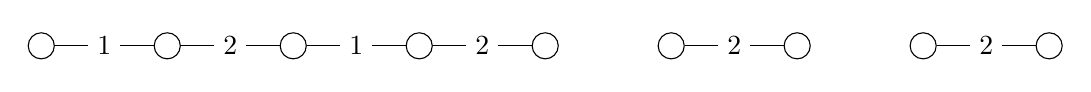
\begin{tikzpicture}[scale=.8]

        \begin{scope}[every node/.style={circle,draw}]
          \node (2)  at (0,0)  {};
          \node (3)  at (2,0)  {};
          \node (4)  at (4,0)  {};
          \node (5)  at (6,0)  {};
          \node (6)  at (8,0)  {};
          \node (7)  at (12,0)  {};
          \node (8)  at (10,0)  {};
          \node (9)  at (16,0)  {};
          \node (10) at (14,0)  {};
        \end{scope}

        \begin{scope}[every node/.style={fill=white}]

          \begin{scope}[every edge/.style={draw}]
            \path (2)  edge node {$1$} (3);
            \path (4)  edge node {$1$} (5);
            \path (3)  edge node {$2$} (4);
            \path (5)  edge node {$2$} (6);
            \path (7)  edge node {$2$} (8);
            \path (9)  edge node {$2$} (10);
          \end{scope}
        \end{scope}

      \end{tikzpicture}
      \caption{Second possibility for $\Gamma_{S_1}$}
    \end{center}
  \end{figure}

  \paragraph{}
  In the first graph, the permutation $(\rho_1 \rho_2)^2 \rho_1$ lets the points of the two isolated edges fixed because the permutation uses $\rho_2$ an even number of times. The points only linked by $\rho_1$ edges remain fixed too. But the point linked by $\rho_2$ edges in the big components are swapped. So it is possible to permute only two $\rho_2$ edges without touching the two others.

  \paragraph{}
  In the second graph, $(\rho_1\rho_2)^4 \rho_1$ gives the same result.

  \paragraph{}
  Now, let's study $S_2$, the disposition of the edges alongside the alternating square is very important. Therefore there are 3 possibilities:

  \begin{figure}[H]
    \begin{center}
      \begin{tikzpicture}[scale=.8]

        \begin{scope}[every node/.style={circle,draw}]
          \node (1)  at (-2,0)  {};
          \node (2)  at (0,0)  {};
          \node (5)  at (2,0)  {};
          \node (6)  at (4,0)  {};
          \node (7)  at (6,0)  {};
          \node (8)  at (6,2)  {};
          \node (9)  at (8,2)  {};
          \node (10) at (8,0)  {};
          \node (11) at (10,0) {};
        \end{scope}

        \begin{scope}[every node/.style={fill=white}]

          \begin{scope}[every edge/.style={draw}]
            \path (1)  edge node {$2$} (2);
            \path (5)  edge node {$2$} (6);
            \path (7)  edge node {$2$} (8);
            \path (9)  edge node {$2$} (10);
            \path (6)  edge node {$3$} (7);
            \path (10) edge node {$3$} (11);
            \path (7)  edge node {$4$} (10);
            \path (8)  edge node {$4$} (9);
          \end{scope}
        \end{scope}

      \end{tikzpicture}
      \caption{First possibility for $\Gamma_{S_2}$}
    \end{center}
  \end{figure}

  \begin{figure}[H]
    \begin{center}
      \begin{tikzpicture}[scale=.8]

        \begin{scope}[every node/.style={circle,draw}]
          \node (1)  at (-2,0)  {};
          \node (2)  at (0,0)  {};
          \node (5)  at (2,0)  {};
          \node (6)  at (4,0)  {};
          \node (7)  at (6,0)  {};
          \node (8)  at (6,2)  {};
          \node (9)  at (8,0)  {};
          \node (10) at (8,2)  {};
          \node (11) at (10,2) {};
        \end{scope}

        \begin{scope}[every node/.style={fill=white}]

          \begin{scope}[every edge/.style={draw}]
            \path (1)  edge node {$2$} (2);
            \path (5)  edge node {$2$} (6);
            \path (7)  edge node {$2$} (8);
            \path (9)  edge node {$2$} (10);
            \path (6)  edge node {$3$} (7);
            \path (10) edge node {$3$} (11);
            \path (7)  edge node {$4$} (9);
            \path (8)  edge node {$4$} (10);
          \end{scope}
        \end{scope}

      \end{tikzpicture}
      \caption{Second possibility for $\Gamma_{S_2}$}
    \end{center}
  \end{figure}

  \begin{figure}[H]
    \begin{center}
      \begin{tikzpicture}[scale=.8]

        \begin{scope}[every node/.style={circle,draw}]
          \node (1)  at (-2,0)  {};
          \node (2)  at (0,0)  {};
          \node (5)  at (2,0)  {};
          \node (6)  at (4,0)  {};
          \node (7)  at (8,2)  {};
          \node (8)  at (6,2)  {};
          \node (9)  at (6,0)  {};
          \node (10) at (8,0)  {};
          \node (11) at (10,0) {};
        \end{scope}

        \begin{scope}[every node/.style={fill=white}]

          \begin{scope}[every edge/.style={draw}]
            \path (1)  edge node {$2$} (2);
            \path (5)  edge node {$2$} (6);
            \path (7)  edge node {$2$} (8);
            \path (9)  edge node {$2$} (10);
            \path (6)  edge node {$3$} (9);
            \path (10) edge node {$3$} (11);
            \path (7)  edge node {$4$} (10);
            \path (8)  edge node {$4$} (9);
          \end{scope}
        \end{scope}

      \end{tikzpicture}
      \caption{Third possibility for $\Gamma_{S_2}$}
    \end{center}
  \end{figure}

  \paragraph{}
  The group generated by the right component is transitive because the component is connected. It's also 2-transitive, this can be checked by fixing the most right point and trying to move it's neighbor. For the first possibility this can be obtained by the permutation $\rho_2 \rho_4 \rho_3 \rho_2 \rho_3 \rho_2 \rho_3$. This can easily be proved for the three graphs and the proof is left to the reader.

  \paragraph{}
  The group is 2-transitive and thus primitive. The list of all primitive groups on seven points can be found in~\cite{buekenhout1996list}. The group is 2-transitive and so its order is a multiple of $7 \times 6 = 42$. But it is possible to find one subgroup by looking at the group generated by $\rho_2$ and $\rho_3$ only. This group is $D_{10}$ which is of order 10. The order of the group must also divide the order of those sub-groups.

  \paragraph{}
  Thus the order of the group must be a multiple of $7 \times 6 \times 5 = 210$. By looking at the list, there are only two primitive groups on seven points such that 210 divides they orders : $A_7$ and $S_7$. But the permutation $\rho_2$ is odd on those seven points, the only possibility is $S_7$.

  \paragraph{}
  But then every $\rho_2$ edge is an involution on those seven points. The other component, that only contains a $\rho_2$ edge must be there to keep the parity of the whole permutation. Therefore this group contains the same involution on four points that was found for $\Gamma_{S_1}$. This involution is in $\Gamma_{S_1}$ and in $\Gamma_{S_2}$ but not in $\Gamma_{\rho_2}$ thus $\Gamma$ does not satisfy the intersection property and is not a C-group.

\end{proof}

\paragraph{}
Now we have proven that there is no abstract polytopes of rank $5$ on $A_{11}$. Next we will prove the same for rank 4.
